\documentclass[5p,11pt,numbers]{elsarticle}
\journal{SoftwareX}
\usepackage{amsmath,amssymb}
\usepackage{booktabs}
\usepackage{graphicx}
\usepackage{tikz}
\usetikzlibrary{positioning}
\usepackage{xurl}
\usepackage{hyperref}
\usepackage{microtype}
\usepackage{lineno}
\usepackage[utf8]{inputenc}
\usepackage[T1]{fontenc}
\usepackage{lmodern}
\graphicspath{{../../figures/}}
\setlength{\emergencystretch}{3em}

\begin{document}
\begin{frontmatter}
\title{WS4: a compiled-state software architecture with exact replay for landscape harvest scheduling}
\author[ubc]{Gregory Paradis}
\affiliation[ubc]{organization={UBC FRESH Lab, University of British Columbia}, country={Canada}}
\ead{gregory.paradis@ubc.ca}

\begin{abstract}
WS4 is an open-source Python system that compiles landscape harvest-scheduling models into a stable
sparse form and searches them with exact accounting. It separates four concerns usually rebuilt
together: a versioned compiled model, compact candidate and sparse effect indexes, exact resident
accounting, and batched GPU search with exact CPU replay. Every reported schedule is replayed through
the exact CPU evaluator that is the evidence authority. On a public frozen TSA24 landscape with 208,255
operable blocks, a 100,000-generation five-seed campaign reaches 512.574--518.621 (mean 515.682), and
all five schedules replay exactly. The level penalty is a normalized mean-level term, not a per-period
floor: the realized level ranges from 51.21 to 52.49M~m\textsuperscript{3} per 10-year period
against a deliberately unattainable 70M aspiration. A 5,000-block diagnostic reduces move-evaluation
time by $2.00\times10^{3}$ with objective agreement to $3.7\times10^{-9}$, and a 64-genome factorized
batch runs 248 times faster on CUDA than on a single-device CPU path. The contribution is the software architecture
and its replay contract; we make no independent harvest-scheduling comparison or state-of-the-art claim.
\end{abstract}

\begin{keyword}
landscape harvest scheduling \sep compiled model \sep GPU population search \sep exact replay \sep reproducibility
\end{keyword}
\end{frontmatter}

\linenumbers
\modulolinenumbers[1]

\section{Motivation and significance}

Landscape harvest scheduling assigns treatments to blocks over time under growth, operability, and
flow objectives. At timber-supply-area scale the state is large and the objective is a weighted
compromise, so exact methods are limited and heuristic search is standard
\citep{johnson1977,davis2001}. The recurring software problem sits beneath the optimisation problem. A
compiled forest model contains blocks, fragments, strata, tracks, treatments, transitions, growth
curves, products, and accounting rules. A search move changes one small part of that model, but
implementations often rebuild a much larger state to evaluate it. The model, the accounting state, and
the move are therefore rebuilt together, which makes experiments slow, replay fragile, and the effect
of a search method hard to separate from an implementation detail.

Harvest-scheduling studies have compared search methods for decades: simulated annealing with spatial
constraints \citep{lockwood1993}, tabu search against a genetic algorithm \citep{boston2002}, and eight
heuristic techniques \citep{bettinger2002}. Reviews document the range of spatial formulations
\citep{murray1999,baskent2005}, and exact approaches remain restricted \citep{goycoolea2005}. These
studies treat the search method as an experimental factor, but each is tied to its own model and
accounting implementation. Reproducibility guidance makes the same point: a result depends on the
compiled model, candidate order, weights, hardware, and replay procedure, not only on a seed and an
objective value \citep{peng2011,sandve2013,wilson2014,stodden2016}.

WS4 (Wood Supply Simulation System) addresses that layer. It compiles a landscape model into versioned
columnar tables, builds a compact candidate index and a sparse effect table, maintains an exact resident
accounting state, runs a batched GPU population search, and replays every reported schedule through an
exact CPU evaluator. The
software is developed by the UBC FRESH Lab. This paper is a software note: it describes the design and
the exact-state contract, illustrates them on one public instance, and states what the evidence does
and does not establish. It makes no environmental-modelling claim, no independent harvest-scheduling
comparison, and no state-of-the-art performance claim.

The intended users are groups with a compiled spatial model who want to vary search operators without
rebuilding accounting, reviewers who need to replay an incumbent, and instructors who need an
inspectable example of exact incremental evaluation.

\section{Software description}

\subsection{Architecture overview}

\begin{figure}[t]
\centering
\resizebox{\linewidth}{!}{%
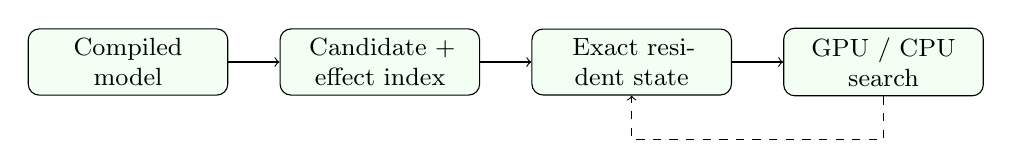
\begin{tikzpicture}[node distance=0.65cm, every node/.style={font=\small}]
\node[draw, rounded corners, fill=green!5, text width=2.3cm, align=center] (raw) {Compiled model};
\node[draw, rounded corners, fill=green!5, text width=2.3cm, align=center, right=of raw] (index) {Candidate + effect index};
\node[draw, rounded corners, fill=green!5, text width=2.3cm, align=center, right=of index] (state) {Exact resident state};
\node[draw, rounded corners, fill=green!5, text width=2.3cm, align=center, right=of state] (search) {GPU / CPU search};
\draw[->] (raw) -- (index);
\draw[->] (index) -- (state);
\draw[->] (state) -- (search);
\draw[->, dashed] (search.south) -- ++(0,-0.55) -| (state.south);
\end{tikzpicture}%
}
\caption{Compiled-state architecture. The resident state is authoritative; search reads and writes it
through exact apply and undo operations.}
\label{fig:architecture}
\end{figure}

The software has four layers (Figure~\ref{fig:architecture}). A compiled model is the stable input. A
candidate index and a sparse effect table make it cheap to query. An exact resident state holds the
realized accounting totals and is the objective authority. A batched GPU population search explores
assignments, and an exact CPU replay path verifies the reported result. The design also supports a
CPU-refinement handoff, in which an elite schedule is loaded into the resident state, improved with
local moves, and written back as a GPU seed; that handoff is designed but is not part of the measured
campaign.

The layers exchange explicit objects rather than implicit global state. The search sees only the
compiled tables, the candidate list, the sparse rows, and the resident state, so it cannot read raw
inventory or mutate accounting outside the apply/undo interface. A run builds or loads the index and
table, initializes the state, runs for a declared budget, writes a record, and replays it through the
exact evaluator. Each stage writes an artifact with an identity, so the next stage can reject a
mismatch.

\subsection{Compiled model and candidate index}

The compiled dataset is the boundary between ingestion and execution. It is a versioned directory of
columnar tables plus a manifest. The tables describe fragments, blocks, tracks, strata, treatments,
curves, features, products, accounts, groups, and compile diagnostics. The manifest records the schema
version, source identities and hashes, compile options, and table list. Compilation happens at the
fragment level; a block is a runtime aggregate of its fragments. The search never reads the raw
inventory or recompiles the recipe. Compile diagnostics, such as blocks with no operable chain and
unreachable transitions, are stored as data so an experiment can state how many blocks were excluded
and why. Compile options are part of the identity because eligibility and operability windows change
the candidate set; two datasets with the same source but different options are different models.

For each block, the candidate index stores the feasible treatment chains in a stable order. A chain is
an ordered sequence of treatment events, each a treatment and a year; the empty chain is included and
is a valid decision. The index is built by walking track transitions from the block's initial state and
applying the compiled windows. The order is part of the contract: the effect table and the search
reference candidate positions, so changing the order changes the meaning of a cached effect. The index
is smaller than the full cross-product but richer than a binary harvest decision.

\subsection{Sparse effect table}

A block/chain pair affects only a small number of \texttt{(year, account)} cells. The effect table
stores, for each block and candidate chain, a sparse row of those cells and their values relative to
the untreated block, plus the empty-schedule base totals and block row starts. A move is therefore
priced by the cells that the old and new chains touch, not by iterating over the whole schedule. Rows
are relative, so apply and undo are an addition and a subtraction rather than a recomputation, and the
base is stored once rather than duplicated for every candidate.

The table has three costs. The build cost is proportional to the number of candidate chains times the
cells per chain and is paid once per dataset and table format. The storage cost is proportional to the
number of non-zero cells, not to the dense block-by-period-by-account product. The query cost for one
move is proportional to the old and new rows. The table identity includes the dataset fingerprint,
candidate order, target-cell geometry, horizon, period width, and table format version. It is a cache
key: a dataset change forces a rebuild, while a change to weights, priorities, or targets is a pricing
change and reuses the table. The identity check is also a failure detector, because a stale table would
attach rows to the wrong model or chains. If the table does not fit in device memory, a population
search cannot run; the TSA24 table uses a lean format that omits the full row index.

\subsection{Exact resident state and objective}

The resident state stores realized totals per \texttt{(period, account)} plus the current chain for each
block. Applying a move subtracts the old row and adds the new row; undo applies the inverse. The
invariant is that the state always equals the empty-schedule base plus the rows of the current
assignment. The update does not depend on move history, so a block that reached a chain after many
toggles contributes exactly what a block that reached it in one step contributes. Compound moves are
decomposed into elementary changes before they reach the state, and the state never stores a
search-specific diff.

The objective is weighted goal programming. Each target contributes a one-sided penalty for falling
below a minimum or exceeding a maximum:
\begin{align}
s_{t,p} &= \max(m_t - v_{t,p}, 0),\\
e_{t,p} &= \max(v_{t,p} - M_t, 0),\\
\tau_{t,p} &= w^-_t\,\phi(s_{t,p}) + w^+_t\,\phi(e_{t,p}),
\end{align}
where $\phi$ is linear or quadratic, $v_{t,p}$ is the realized value of target $t$ in period $p$, and
$m_t$ and $M_t$ are the hinge values. The target set is not a set of hard constraints: ``minimum'' and
``maximum'' name the hinge of the penalty, not a feasible interval.

The TSA24 target has two roles. One even-flow target spans periods 1--20, compares each period with
the reference period, and charges a squared deviation outside a $\pm1\%$ band with weight 10,000.
Second, the level target is a normalized linear penalty on the mean realized level over the twenty
periods:
\begin{equation}
\ell = 20 \times 100 \times \frac{70{,}000{,}000 - \bar v}{70{,}000{,}000},
\label{eq:level}
\end{equation}
where $\bar v$ is the mean realized level in m\textsuperscript{3} per 10-year period and
70,000,000~m\textsuperscript{3} is the aspiration. The level term is dimensionless and is scaled by the
number of periods; it is not a per-period hard floor. The aspiration is deliberately above the level
the estate is expected to achieve, so it creates a common pull-up gradient. The even-flow target selects
the flattest profile at the level where the two roles reach their best weighted compromise. The
realized level is an outcome, not a declared feasible floor.

For a move on block $b$ from chain $c_{\mathrm{old}}$ to chain $c_{\mathrm{new}}$, let $p$ be the sparse
pending change to the realized account totals and let $\mathcal{T}$ be the targets it affects. The
objective delta is
\begin{equation}
\Delta Z_b(c_{\mathrm{old}}\!\to c_{\mathrm{new}})
= \sum_{t\in\mathcal{T}}\left[\pi_t(T+p)-\pi_t(T)\right],
\label{eq:delta}
\end{equation}
where $\pi_t$ is the target's penalty function and $T$ is the current state. For a linear level target,
$\pi_t$ is a per-cell penalty. For the even-flow target, $\pi_t$ is a penalty over the period vector, so
the delta re-evaluates the affected flow target rather than summing independent cell penalties. The
cost is proportional to the pending cells plus the flow target's period vector, not to the number of
blocks in the schedule. The implementation uses this identity in the local-search paths and retains a
whole-schedule evaluator as a reference.

A schedule is feasible when every operable block has one candidate chain and the chain's events obey the
compiled windows; a feasible schedule can still miss every target, because the objective is a weighted
penalty, not a feasibility measure. The search uses four move families: toggle a chain, shift an event,
swap chains between blocks, and destroy-and-repair a small set. The first three are local and
reversible; the fourth is decomposed into local changes. The replay contract applies to the final
assignment, not the move decomposition.

\subsection{GPU population search and exact replay}

The GPU population evaluates a batch of candidate-index genomes against the sparse table. The batch is
a matrix of block/chain choices; the kernel accumulates the corresponding rows into a per-genome
objective. The device path produces a ranking and does not update the resident state. The CPU path
reconstructs the state from the stored assignment and computes the objective with the same accounting
rules. The two paths can differ in floating-point order, so the record stores the CPU replay objective,
not the device objective. A small device/CPU difference is acceptable as a search signal; it is not
acceptable as a reported result.

Every reported schedule is stored as a complete block/treatment/offset assignment. The record carries
the instance and its availability, the objective and feasibility definition, the algorithm, version,
and configuration, the seed, the hardware and software, the wall and search times, the schedule path
and SHA-256, the exact-replay flag, and the per-target residuals. A validator checks the schema, the
schedule path, and the hash. The replay gate is a separate program: it loads the compiled model, reads
the stored schedule, validates coverage and candidate membership, and evaluates the objective without
calling the optimizer. It verifies the incumbent, not the search trajectory, and does not prove that
the search explored the neighbourhood it claims.

The software therefore supports two levels of reproducibility. The search is reproducible from its
configuration and seed for a fixed implementation, and the reported result is replayable from the
stored schedule even if the search is not rerun. The record format also permits a table to be
regenerated from the record files rather than typed by hand. Four failure modes are exposed: a model
change without a table rebuild, an irreversible move, a reported device objective, and a partial or
infeasible schedule. None is silent in a record that passes the gate. The gate does not catch a bad
search design: a poor schedule can still produce an exact, replayable record. The harness guarantees
the evidence; the experiment argues about the search.

\subsection{Implementation and use}

The implementation is in Python 3.12 and uses NumPy \citep{harris2020}, SciPy \citep{virtanen2020},
Numba for optional acceleration \citep{lam2015}, and PyTorch for the GPU path \citep{paszke2019}. The
reported campaign ran on an NVIDIA RTX PRO 6000 Blackwell Max-Q Workstation Edition (97,887~MiB) with
an Intel Xeon Gold 6254 CPU at 3.10~GHz, Python 3.12.3, and WS4 release candidate \texttt{ws4-v0.2.0-p14rc1}
\citep{ws4}. The command-line surface is small: compile a dataset, build an effect table, run a search
with a configuration file, and replay a record. The test suite covers the compiled-table schema,
candidate index, effect rows, apply/undo invariants, evaluator, and record validator. The large GPU
effect table and caches are not part of the small public dataset artifact; they are rebuilt from the
published recipe.

\section{Validation and illustration}

\subsection{Instance and target}

The case study uses the public frozen artifact \texttt{ws4-tsa24-evenflow-v1}, a TSA24/Prince George
landscape compiled for WS4 \citep{tsa24artifact}. The compiled dataset contains 458,708 blocks; 208,255
have at least one operable treatment chain and form the search universe. The horizon is 200 years,
divided into twenty 10-year accounting periods. The initial schedule is the oldest-first seed from the
artifact. It is feasible but is not an optimised control; its objective is 1,722,140,000, dominated by
even-flow deviations.

The target combines the weight-10,000 even-flow band with the weight-100 level term of
Equation~\ref{eq:level}. The 70M~m\textsuperscript{3} per-period aspiration is above the attainable
level by design: it is a pull-up gradient, not a feasibility constraint. The reported run has no hard
spatial constraints; it is not a test of adjacency or opening-size feasibility. A reader can obtain the
same blocks, target, and initial schedule, and the compiled build is a derived artifact with its own
terms. The instance is large enough to exercise the compiled boundary and small enough to run a
100,000-generation campaign on one workstation. That combination is why it is used, not a claim that
TSA24 represents all timber supply areas.

\subsection{Scaling from 1,000 to 100,000 generations}

Table~\ref{tab:scaling} reports the seed-7 runs at three budgets. The 1,000-generation run reduced the
objective from 1,722,140,000 to 8,588,730 in 9.38~s of search time (23.1~s wall). The 10,000-generation
run reached 76,540.7 in 89.8~s search (157~s wall). The 100,000-generation run reached 517.862 in
856~s search (942~s wall). Wall time includes model and cache setup; search time is the GPU budget.

The objective falls by roughly two orders of magnitude from 1,000 to 10,000 generations and by another
two orders from 10,000 to 100,000 (Figure~\ref{fig:scaling}). That is not a convergence proof; it shows
that the search is still making progress at the largest budget. The flow term collapses faster than the
level term, because the even-flow target is what the population can improve by reshaping the profile.
The level term remains between 499.821 and 517.290 because the aspiration is above the achievable level,
not because the search ignores it. A 1,000-generation run is a smoke test and a scaling anchor, not a
competitive result; the three budgets make that sensitivity visible.

\begin{table}[t]
\centering
\caption{Seed-7 scaling on the frozen TSA24 instance. Wall time includes model and cache setup; search
time is the GPU search budget.}
\label{tab:scaling}
\small
\resizebox{\linewidth}{!}{%
\begin{tabular}{rrrrr}
\toprule
Generations & Objective & Flow term & Level term & Search / wall (s) \\
\midrule
1,000 & 8,588,730 & 8,588,230 & 499.821 & 9.38 / 23.1 \\
10,000 & 76,540.7 & 76,026.9 & 513.832 & 89.8 / 157 \\
100,000 & 517.862 & 2.721 & 515.141 & 856 / 942 \\
\bottomrule
\end{tabular}%
}
\end{table}

\begin{figure}[t]
\centering
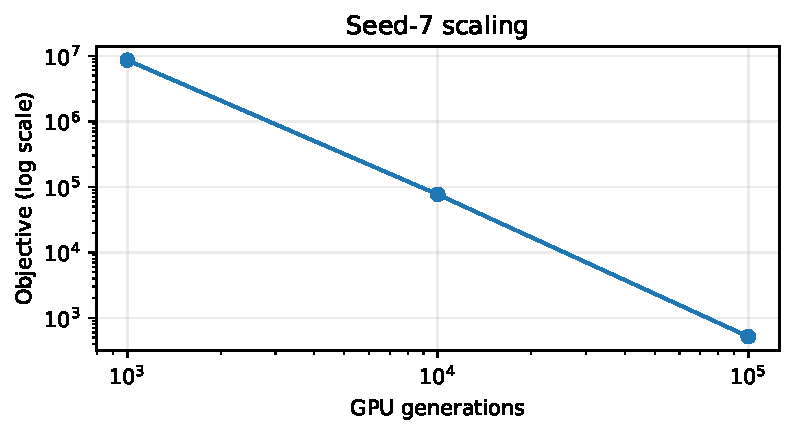
\includegraphics[width=0.68\linewidth]{scaling.pdf}
\caption{Seed-7 scaling from 1,000 to 100,000 GPU generations. Both axes are logarithmic.}
\label{fig:scaling}
\end{figure}

\subsection{Five-seed campaign}

Table~\ref{tab:seeds} reports the five-seed campaign at 100,000 generations. The best objective is
512.574, the worst is 518.621, the mean is 515.682, and the median is 515.938. Seed~7, the scaling
reference, lies at 517.862 and is not part of the five-seed summary. All five campaign schedules replay
exactly, and the campaign took $4.00\times10^{3}$~s wall for all five runs.

The realized level is approximately 51.21--52.49M~m\textsuperscript{3} per 10-year period against the
70M aspiration. The level term is therefore the dominant part of the final objective, not a residual
that the search failed to remove. The initial seed is dominated by flow deviations; the final schedules
have almost no flow penalty but still pay for the level aspiration. Reporting the split prevents a
reader from inferring that the target was nearly satisfied. The five-seed spread is small in objective,
but the seeds do not all reach the same flow/level compromise. The mean and median are descriptive
statistics for five runs, not a confidence interval or a test against a baseline.

\begin{table}[t]
\centering
\caption{Five-seed 100,000-generation campaign. All objectives are exact CPU replays; the mean and
median in the text use these five seeds.}
\label{tab:seeds}
\small
\resizebox{\linewidth}{!}{%
\begin{tabular}{rrrrr}
\toprule
Seed & Objective & Flow term & Level term & Realized level (M~m\textsuperscript{3}/period) \\
\midrule
1 & 518.621 & 1.331 & 517.290 & 51.21--52.25 \\
2 & 512.574 & 0.000 & 512.574 & 51.46--52.49 \\
3 & 515.938 & 0.000 & 515.938 & 51.31--52.32 \\
4 & 514.746 & 0.000 & 514.746 & 51.34--52.35 \\
5 & 516.530 & 0.076 & 516.454 & 51.26--52.29 \\
\bottomrule
\end{tabular}%
}
\end{table}

\subsection{Evaluation path and batch microbenchmark}

A full-instance whole-schedule ablation is impractical, because a single full evaluation of the
208,255-block schedule is the motivating cost. We therefore report a disclosed diagnostic on the first
5,000 blocks of the recorded 100,000-generation seed-7 schedule, over 50 moves. A cold whole-schedule
evaluation took 54.8~s; after warm-up, a whole-schedule move evaluation took 1.09~s. Exact incremental
delta plus apply took 0.542~ms per move, a factor of $2.00\times10^{3}$. The final incremental objective
matched the whole-schedule objective to $3.7\times10^{-9}$ (Table~\ref{tab:eval}). The subset is not a
random sample, and the 50 moves are a diagnostic sequence rather than a search trajectory. The result
isolates the evaluation path from the GPU population search; it is not a full-instance ablation and
does not measure a matched CPU search.

\begin{table}[t]
\centering
\caption{Evaluation-path diagnostic on the first 5,000 blocks of the recorded 100,000-generation seed-7
schedule, 50 moves. Times are exact CPU measurements; relative time is warm whole-schedule move time
divided by the row time.}
\label{tab:eval}
\small
\resizebox{\linewidth}{!}{%
\begin{tabular}{@{}llrrr@{}}
\toprule
Path & Measurement & Time & Relative & Error \\
\midrule
Whole schedule, cold & first evaluation & 54.8~s & -- & -- \\
Whole schedule, warm & mean per move & 1.09~s & 1 & -- \\
Incremental delta + apply & mean per move & 0.542~ms & $2.00\times10^{3}$ & $3.7\times10^{-9}$ \\
\bottomrule
\end{tabular}%
}
\end{table}

A second check evaluates the same 64-genome batch against four mixed feature/product cells on CPU and
CUDA, using the TSA24 factorized archive. The CPU batch takes 23.1~s and the CUDA batch 0.0931~s, a
factor of 248; throughput is 2.77 and 687 genomes/s. The maximum absolute error against the exact
evaluator is $1.71\times10^{-6}$ on both paths. The factorized build takes 234~s and the GPU peak
allocation is 9.27~GB. This is a batch microbenchmark, not an end-to-end search comparison and not
evidence that the architecture causes a search-speed gain. The CPU path is a single-device tensor path,
not a tuned multithreaded batch, and the build cost matters only when the table is reused.

\subsection{What the validation establishes}

The results establish that the software can run a 208,255-operable-block instance at a
100,000-generation GPU budget and produce exact, replayable schedules; that the sparse table plus
resident state avoids a full re-simulation without changing the objective; and that the factorized GPU
batch evaluates a population quickly on this instance. They do not establish a controlled
architecture-versus-implementation effect, an independent quality comparison, a tuned CPU/GPU ranking,
or optimality. The retained CPU simulated-annealing run is untuned, single-seed, and not equal-work; it
is not used here as a quality baseline.

\section{Impact}

The immediate software impact is measured in exact replay and reduced evaluation cost, not in adoption numbers: a 100,000-generation campaign is replayable from stored assignments, and a move evaluation drops from 1.09~s to 0.542~ms on the diagnostic subset. The architecture is reusable when the model boundary is the expensive part of a project. A team with a
compiled model and an exact evaluator can add a candidate index and a sparse effect table without
changing model semantics. A team with a fast heuristic but no replay contract can wrap the heuristic in
the adapter and keep the evidence boundary. A team comparing search methods can hold the model and
target fixed and vary only the search layer. Because weights are data, a sensitivity study can reuse the
table and recompute only pricing. Adapting to a new model requires a compiler that emits the tables and
manifest, a candidate-index builder for the model's eligibility rules, and an effect-row builder that
maps a block/chain pair to target cells. The state, search loop, record schema, and replay gate are
designed to be model-agnostic.

\subsection{Reuse potential}

A practical integration pattern follows: freeze the compiled model and record its fingerprint; freeze
the candidate order and target file; build the table once and record its identity; run with a declared
population, budget, and seed; store the assignment, not only the seed; replay it through the exact
evaluator; and report the stop reason with the result. The replay gate also supports archival review: a
repository can store the assignment and record, and a future reader can verify the objective without
rerunning the search or needing the original GPU.

\subsection{Limitations}

The limitations are explicit. The validation covers one landscape, one target construction, and one
20-period horizon. The reported run has no hard adjacency or opening-size constraints, so the software
is not validated on the spatial-constraint case that motivates much of the literature. There is no
independent harvest-scheduling model or LP/MIP bound on the same instance, so the objective values are
not a competitive quality result. The five-seed campaign is descriptive; the evaluation-path ablation
uses a 5,000-block subset; and the factorized result is a 64-genome batch microbenchmark. A tuned CPU-GA
at equal work, a full-instance evaluation-path comparison, and a cache-load/search split remain open.

Two constraints follow. The effect table must fit in device memory alongside the population batch; the
campaign required a multi-gigabyte device allocation, and a larger candidate set would need a different
partitioning. The GPU code is public as release candidate \texttt{ws4-v0.2.0-p14rc1}; the paper-specific
schedules and replay scripts are in the public papers repository under release candidate
\texttt{p14-evidence-rc3}. The release is a public snapshot; a DOI is still pending, so the replay
contract is not yet an archival DOI service. The target
construction is also a policy choice: the software can make it exact and replayable, not correct, and
the TSA24 configuration is not an operational decision.

\section{Conclusions}

WS4 turns a compiled landscape model into a stable sparse representation, maintains exact resident
accounting, searches with a batched GPU population, and replays every reported schedule through an
exact CPU evaluator. On the public TSA24 instance, the software completes a 100,000-generation,
five-seed campaign on 208,255 operable blocks, and all five incumbents replay exactly. The diagnostic
measurements show that a move can be priced from a sparse effect row instead of a whole-schedule
re-simulation, with objective agreement at $3.7\times10^{-9}$.

The contribution is the software architecture and its evidence boundary, not a new metaheuristic or a
landscape-quality claim. The next steps are a DOI and a tested one-command
replay, a tuned CPU comparison at equal work, a full-instance evaluation-path study, and a
spatial-constraint extension. Until those exist, the software is an exact, replayable platform for
controlled landscape-search experiments, not a leaderboard entry. It is a reproducible case, not a
competitive solver.

\clearpage
\section*{Code metadata}

\begin{table}[!h]
\centering
\small
\resizebox{\linewidth}{!}{%
\begin{tabular}{@{}lp{11.2cm}@{}}
\toprule
Nr. & Code metadata description \\
\midrule
C1 & Current code version: \texttt{ws4-v0.2.0-p14rc1} (public prerelease) \\
C2 & Permanent link to code/repository: \newline \url{https://github.com/UBC-FRESH/ws4/releases/tag/ws4-v0.2.0-p14rc1} \\
C3 & Legal code licence: Apache-2.0 for WS4; the TSA24 artifact retains its own public terms \\
C4 & Code versioning system: Git \\
C5 & Software code languages and tools: Python 3.12; NumPy; PyTorch (CUDA); Numba (optional) \\
C6 & Compilation requirements, operating environments, and dependencies: Linux; Python 3.12.3; CUDA-capable GPU with multi-gigabyte memory (9.27~GB peak in the factorized batch); virtual-environment install \\
C7 & Link to developer documentation: \url{https://github.com/UBC-FRESH/ws4} \\
C8 & Test command: \texttt{python -m pytest}; replay: \texttt{WS4\_ROOT=... TSA24\_ROOT=... FHOPS\_ROOT=... bash paper/replay\_all.sh} \\
C9 & Support email: \url{mailto:gregory.paradis@ubc.ca} \\
\bottomrule
\end{tabular}%
}
\caption{Code metadata (mandatory).}
\label{tab:metadata}
\end{table}

\section*{Data and code availability}

The TSA24 benchmark artifact is available at
\url{https://github.com/UBC-FRESH/femic-tsa24-instance/releases/tag/ws4-tsa24-evenflow-v1}. The build
and replay recipe is in \texttt{BENCHMARK\_ARTIFACT.md} in that repository. The paper-specific
schedules and replay scripts are in the public evidence release
\url{https://github.com/UBC-FRESH/fresh-solutions-papers/releases/tag/p14-evidence-rc3}; a DOI
remains pending.

\bibliographystyle{elsarticle-num}
\bibliography{references-softwarex}

\end{document}
